\documentclass[a4paper, 12pt]{report}
%Packages
\usepackage[T1]{fontenc}
\usepackage[ngerman]{babel}
\usepackage{hyphenat}
\usepackage{graphicx}
\usepackage{amsmath}
\usepackage[hidelinks]{hyperref}
\usepackage{siunitx}
\usepackage{titlesec}
\usepackage{setspace}
\usepackage[titles]{tocloft}
\usepackage{multirow}
\usepackage[style=apa, sortcites, url=true]{biblatex}


%Settings
%Change depth of section numbers (1.1.1.1)
\setcounter{secnumdepth}{4}
%Hyphenation for special words
\hyphenation{Mathe-matik wieder-gewinnen}
%Path to images
\graphicspath{ {images/} }
%Set font to Times
\usepackage{mathptmx}
%Change fontsize according to Word template
\makeatletter %only needed in preamble
\renewcommand\Huge{\@setfontsize\Huge{26pt}{39}}
\renewcommand\Large{\@setfontsize\Large{14pt}{21}}
\renewcommand\large{\@setfontsize\large{13pt}{19.5}}
\makeatother

%Change chapter anc section styles
\titleformat{\chapter}[hang] 
{\Large\bfseries}{\thechapter}{1em}{}
\titleformat*{\section}{\large\bfseries}
\titleformat*{\subsection}{\normalsize\bfseries}
\titleformat*{\subsubsection}{\normalsize\bfseries\itshape}
\titleformat*{\paragraph}{\normalsize\bfseries}
\titleformat*{\subparagraph}{\normalsize\bfseries}

%Set spacing
\onehalfspacing

%Table of content settings
\setcounter{tocdepth}{4}
\renewcommand{\cftchapfont}{\normalfont}% titles in bold
\renewcommand{\cftchappagefont}{\normalfont}% page numbers in bold
\renewcommand{\cftdotsep}{1}
\renewcommand{\cftchapleader}{\cftdotfill{\cftsecdotsep}}% dot leaders in bold

%References
\addbibresource{sample.bib}

% Attributes for title page
\title{Titel der Thesis/Hausarbeit}
\author{Hans Student}
\date{31. Oktober 2016}


\begin{document}
	%Title Page
	% Title Page
\begin{titlepage}
	\centering
	Johann Wolfgang Goethe-Universität Frankfurt am Main
	
	Institut für Sportwissenschaften
	
	\vspace{12pt}
	
	Hausarbeit zum Seminar „XY“/Thesis zur Erlangung des Bachelor of Arts im Fach Sportwissenschaften
	
	SS 2015
	
	Dozent/Betreuer: Prof. Dr. Peter Mustermann
	
	\vfill
	
	\begin{flushleft}
		Hans Student, BA, 5 \\ 
		Matrikel-Nr.: 999999 \\ 
		musterstudent@stud.uni-frankfurt.de \\ 
		Frankfurt, den 31. Oktober 2016
	\end{flushleft}
\end{titlepage}

	%Set pagenumbering to Roman style and start with number II for lists
	\pagenumbering{Roman}
	\setcounter{page}{2}
	%Table of contents
	\tableofcontents
	\newpage
	%List of figures
	\listoffigures
	\newpage
	%List of tables
	\listoftables
	\newpage	
	%Set pagenumbering to arabic style for content
	\pagenumbering{arabic}
	%Add includes for chapters
	\chapter{Problemstellung}
Die Problemstellung beinhaltet die Problemhinführung und Formulierung der allgemeinen Fragestellung, die Beschreibung der Ziele der Arbeit sowie eine Übersicht über die Vorgehensweise und Struktur der Arbeit. Sie kann in 1.1 Theoretische Grundlagen bzw. 1.2 Forschungshypothesen unterteilt werden.
\section{Theoretische Grundlagen}
\subsection{Theoretischer Hintergrund}
Hier wird bspw. der theoretische Hintergrund beschrieben.

\subsection{Forschungsstand}
\subsubsection{Aktueller Forschungsstand}
Hier stehen die Ausführungen zum aktuellen Forschungsstand.

\subsubsection{Historischer Forschungsstand}
Hier stehen die Ausführungen zum historischen Forschungsstand.

\section{Forschungshypothesen}
Hier werden die Forschungshypothesen aufgestellt und begründet.
	\chapter{Methoden}
Der Methodenteil kann folgende Punkte beinhalten:
\begin{itemize}
	\item Untersuchungsdesign bzw. Versuchsplan
	\item Überlegungen zu Konsequenzen für die Validität der Untersuchungsergebnisse
	\begin{itemize}
		\item interne Validität
		\item externe Validität
	\end{itemize}
	\item Methodik der Datenerhebung (Personen-/Merkmalsstichprobe und Erhebungsver-fahren sowie Überlegungen zu Konsequenzen für die Repräsentativität der Ergeb-nisse und für Fehler bzw. Gütekriterien der Messungen)
	\item Methodik der Datenauswertung (Datenaufbereitung, ggf. Auswahl der Methoden der statistischen Datenverarbeitung unter Beachtung der Anwendungsvorausset-zungen und Festlegung des Signifikanzniveaus) oder Beschreibung der qualitati-ven Analysemethoden.
\end{itemize}

	\chapter{Ergebnisse}
Die Ergebnisteil kann sich in (1) Beschreibung der Ergebnisse ohne Vorgriff auf die Interpretation oder Diskussion sowie (2) ggf. in die Darstellung der in der Untersuchung erhobenen Ergebnisse in anschaulicher Form (z. B. Tabellen, Abbildungen) gliedern. Es empfiehlt sich häufig eine dreistufige Vorgehensweise:
\begin{enumerate}
	\item deskriptive Statistik (zur Beschreibung der abhängigen oder unabhängigen Variable für die gesamte Stichprobe)
	\item Inferenzstatistik (Hypothesentestung, z. B. getrennt nach unabhängigen Variablen)
	\item weiterführende Analysen (z. B. Prüfung des Einflusses von Kontrollvariablen oder des Zusammenhangs von abhängigen Variablen)
	Zur besseren Veranschaulichung können Abbildungen wie folgt verwendet werden:	
\end{enumerate}
\begin{figure}[h]
	\centering
	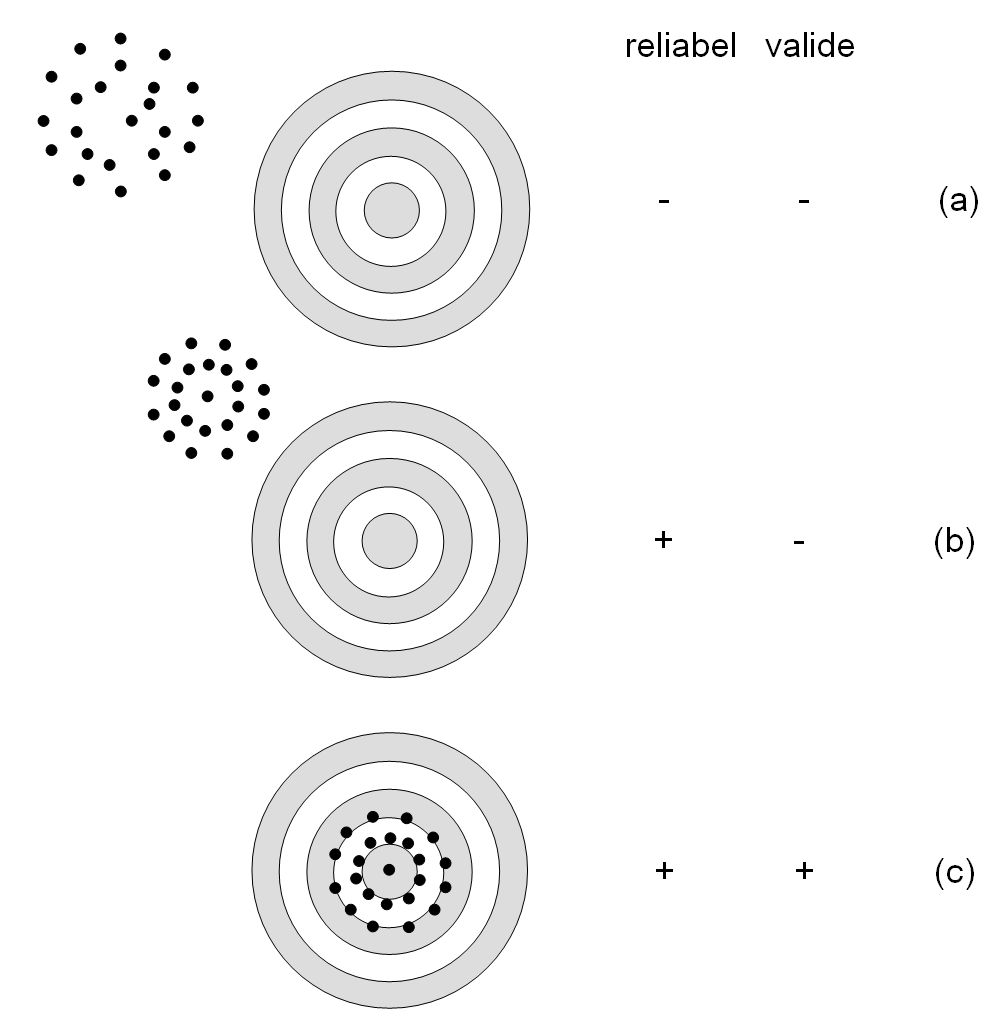
\includegraphics[width=0.7\linewidth]{images/guetekriterien-reliabilitaet-und-variabilitaet}
	\caption{Verdeutlichung der Gütekriterien Reliabilität und Validität (Bös, Hänsel \& Schott, 2004, S. 23).}
	\label{fig:guetekriterien-reliabilitaet-und-variabilitaet}
\end{figure}
Tabellen werden dagegen so verwendet:

	\chapter{Diskussion}
Hier erfolgt die Diskussion und Interpretation der Ergebnisse sowie die Beantwortung der Forschungsfrage (ggf. Hypothesenentscheidung) mit:
\begin{itemize}
	\item Einbezug der forschungsmethodologischen Besonderheiten der Untersuchung: z. B. Bezug auf Gütekriterien der Messungen, interne und externe Validität
	\item Bezug zur Literaturanalyse: Diskussion der Ergebnisse vor dem Hintergrund der im Theorieteil dargestellten Grundlagen und problemrelevanten Forschungsergebnisse
	\item Rückschluss auf die Problem- und Fragestellung: problem- und praxisrelevante Folgerungen aus den Ergebnissen (z. B. Folgerungen für die Trainingspraxis in trainingswissenschaftlichen Untersuchungen)
\end{itemize}
Ein weiterer Inhalt kann der sog. \emph{Ausblick} sein, mit:
\begin{itemize}
	\item Verweis auf ungeklärte Probleme,
	\item Wertung der Arbeit in Hinblick auf zukünftige Forschungsansätze sowie
	\item das Aufzeigen von Forschungsperspektiven.
\end{itemize}


	\chapter{Zusammenfassung}
Hier sollte ein zusammenfassender Überblick über die wichtigsten Aussagen der einzelnen Kapitel der Arbeit stehen. Dieser sollte ohne jede Kenntnis des gesamten Textes verständlich sein und keine neuen Aspekte aufgreifen.
	%References
	\printbibliography[title=Literaturverzeichnis]
	%Appendix
	\addcontentsline{toc}{chapter}{Anhang}
\chapter*{Anhang}
Hier stehen die Anhangstexte, -tabellen, -abbildungen usw.
	%Declaration
	\addcontentsline{toc}{chapter}{Erklärung zur Originalität der Arbeit}
\markboth{Erklärung zur Originalität der Arbeit}{}
\chapter*{Erklärung zur Originalität der Arbeit}
Ich versichere hiermit, dass ich die Arbeit selbstständig verfasst, keine anderen, als die angegebenen Hilfsmittel verwendet und die Stellen, die anderen Werken im Wortlaut oder dem Sinn nach entnommen sind, mit Quellenangaben kenntlich gemacht habe. Dies gilt auch für Zeichnungen, Skizzen, Ton- und Bildträger sowie bildliche Darstellungen.

Die Arbeit wurde bisher (keiner anderen Prüfungsbehörde), weder in identischer, noch in abgewandelter Form, vorgelegt und auch noch nicht veröffentlicht.

\end{document}          
